\begin{example} % EXAMPLE
Approximate the area of the region under $y=4x-x^2$ on the interval $[0,4]$ using $L_4$, $R_4$, and $M_4$. 

\solution We partition the interval $[0,4]$ into the four subintervals $[0,1]$, $[1,2]$, $[2,3]$, and $[3,4]$. In Figure~\ref{fig:apex_5-3_Area1}-(a) we see $4$ rectangles drawn on $f(x) = 4x-x^2$ using the $L_4$. Note how in the first subinterval, $[0,1]$, the rectangle has height $f(0)=0$. We add up the areas of each rectangle, which is width $\times$ height, for our $L_4$ approximation:
\begin{eqnarray*}
L_4 & = & 1 \cdot f(0) + 1 \cdot f(1)+ 1 \cdot f(2) + 1 \cdot f(3) \\
& = & 0+3+4+3 \\
& = & 10.
\end{eqnarray*}
	
Figure~\ref{fig:apex_5-3_Area1}-(b) shows $4$ rectangles drawn under $f$ using $R_4$; note how the rectangle on the subinterval $[3,4]$ has height $0$.  Our approximation gives the same answer as before, though calculated a different way:
\begin{eqnarray*}
R_4 & = & 1 \cdot f(1) + 1 \cdot f(2)+ 1 \cdot f(3) + 1 \cdot f(4) \\
& = & 3+4+3+0 \\
& = & 10.
\end{eqnarray*}

Figure~\ref{fig:apex_5-3_Area1}-(c) shows $4$ rectangles drawn under $f$ using $M_4$. Notice that the height of each of the rectangles is determined by the point in the middle of each subinterval, which are $0.5$, $1.5$, $2.5$, and $3.5$. So
\begin{eqnarray*}
M_4 & = & 1 \cdot f(0.5) + 1 \cdot f(1.5)+ 1 \cdot f(2.5) + 1 \cdot f(3.5) \\
& = & 1.75 + 3.75 + 3.75 + 1.75 \\
& = & 11.
\end{eqnarray*}
\end{example}

\begin{marginfigure} % MARGIN FIGURE
\begin{center}
%\captionsetup[subfigure]{labelformat=empty}
\subfloat[$L_n$]{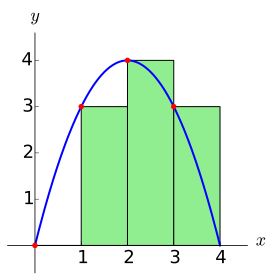
\includegraphics[scale=.5]{figs/4/apex_5-3_Area1Ln.pdf}}
%\caption{Approximating the area under $y=4x-x^2$ on $[0,4]$ using $L_n$} \label{fig:apex_5-3_Area1}

\subfloat[$R_n$]{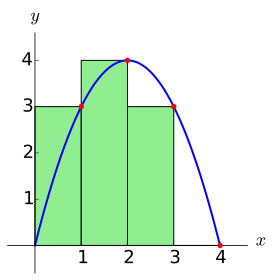
\includegraphics[scale=.5]{figs/4/apex_5-3_Area1Rn.pdf}}
%\caption{Approximating the area under $y=4x-x^2$ on $[0,4]$ using $R_n$} \label{fig:apex_5-3_Area1}

\subfloat[$M_n$]{\includegraphics[scale=.5]{figs/4/apex_5-3_Area1Mn.pdf}}
\caption{Approximating the area under $y=4x-x^2$ on $[0,4]$ using $L_n$, $R_n$, and $M_n$} \label{fig:apex_5-3_Area1}
\end{center}
\end{marginfigure}